\documentclass{article} % For LaTeX2e
\usepackage{nips14submit_e,times}
\usepackage{amsmath}
\usepackage{amsthm}
\usepackage{amssymb}
\usepackage{mathtools}
\usepackage{hyperref}
\usepackage{url}
\usepackage{algorithm}
\usepackage[noend]{algpseudocode}
%\documentstyle[nips14submit_09,times,art10]{article} % For LaTeX 2.09

\usepackage{mathrsfs}
\usepackage{graphicx}
\usepackage{caption}
\usepackage{subcaption}

\def\eQb#1\eQe{\begin{eqnarray*}#1\end{eqnarray*}}
\def\eQnb#1\eQne{\begin{eqnarray}#1\end{eqnarray}}
\providecommand{\e}[1]{\ensuremath{\times 10^{#1}}}
\providecommand{\pb}[0]{\pagebreak}

\newcommand{\E}{\mathrm{E}}
\newcommand{\Var}{\mathrm{Var}}
\newcommand{\Cov}{\mathrm{Cov}}

\def\Qb#1\Qe{\begin{question}#1\end{question}}
\def\Sb#1\Se{\begin{solution}#1\end{solution}}

\newenvironment{claim}[1]{\par\noindent\underline{Claim:}\space#1}{}
\newtheoremstyle{quest}{\topsep}{\topsep}{}{}{\bfseries}{}{ }{\thmname{#1}\thmnote{ #3}.}
\theoremstyle{quest}
\newtheorem*{definition}{Definition}
\newtheorem*{theorem}{Theorem}
\newtheorem*{lemma}{Lemma}
\newtheorem*{question}{Question}
\newtheorem*{preposition}{Preposition}
\newtheorem*{exercise}{Exercise}
\newtheorem*{challengeproblem}{Challenge Problem}
\newtheorem*{solution}{Solution}
\newtheorem*{remark}{Remark}
\usepackage{verbatimbox}
\usepackage{listings}
\title{Linear Algebra II: \\
Problem Set III}


\author{
Youngduck Choi \\
CIMS \\
New York University\\
\texttt{yc1104@nyu.edu} \\
}


% The \author macro works with any number of authors. There are two commands
% used to separate the names and addresses of multiple authors: \And and \AND.
%
% Using \And between authors leaves it to \LaTeX{} to determine where to break
% the lines. Using \AND forces a linebreak at that point. So, if \LaTeX{}
% puts 3 of 4 authors names on the first line, and the last on the second
% line, try using \AND instead of \And before the third author name.

\newcommand{\fix}{\marginpar{FIX}}
\newcommand{\new}{\marginpar{NEW}}

\nipsfinalcopy % Uncomment for camera-ready version

\begin{document}


\maketitle

\begin{abstract}
This work contains solutions to the problem set III
of Linear Algebra II 2016 at Courant Institute of Mathematical Sciences.
\end{abstract}

\bigskip

\begin{question}[1]
\hfill
\begin{figure}[h!]
  \centering
    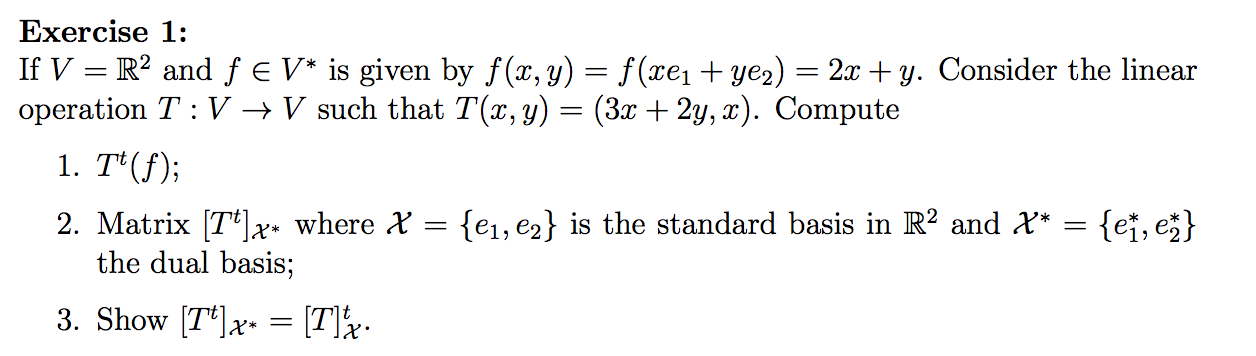
\includegraphics[width=1\textwidth]{LA-3-1.png}
\end{figure}
\end{question}
\begin{solution} \hfill \\
\textbf{(1)}
By the definition of a transpose map, it follows that 
\eQb
T^{t}(f)(x,y) &=& fT(x,y) \\
&=& f(3x+2y,x) = 7x + 4y.
\eQe

\smallskip

\textbf{(2)} From the Theorem 2.25, it follows that the matrix of a transpose map
with respect to the standard basis is the transpose of a matrix with respect to the 
standard basis. We compute the matrix in the next section.

\smallskip

\textbf{(3)} We have
\eQb
T(1,0) &=& (3,1) = 3(1,0) + 1(0,1) \\
T(0,1) &=& (2,0) = 2(1,0) + 0(0,0).
\eQe
It follows that
\eQb 
[T]_{\mathscr{X}} &=& \begin{pmatrix}
3 & 2 \\
1 & 0 \\
\end{pmatrix}, \\
\eQe
which consequently gives
\eQb
[T]_{\mathscr{X}}^t &=& \begin{pmatrix}
3 & 1 \\
2 & 0 \\
\end{pmatrix}. 
\eQe 
Hence, we have shown that $[T^t]_{\mathscr{X}^*} = [T]^t_{\mathscr{X}}$, which is to be 
expected from the Theorem $2.25$, pg.121, in Friedberg. 
\hfill $\qed$
\end{solution}

\newpage

\begin{question}[2]
\hfill
\begin{figure}[h!]
  \centering
    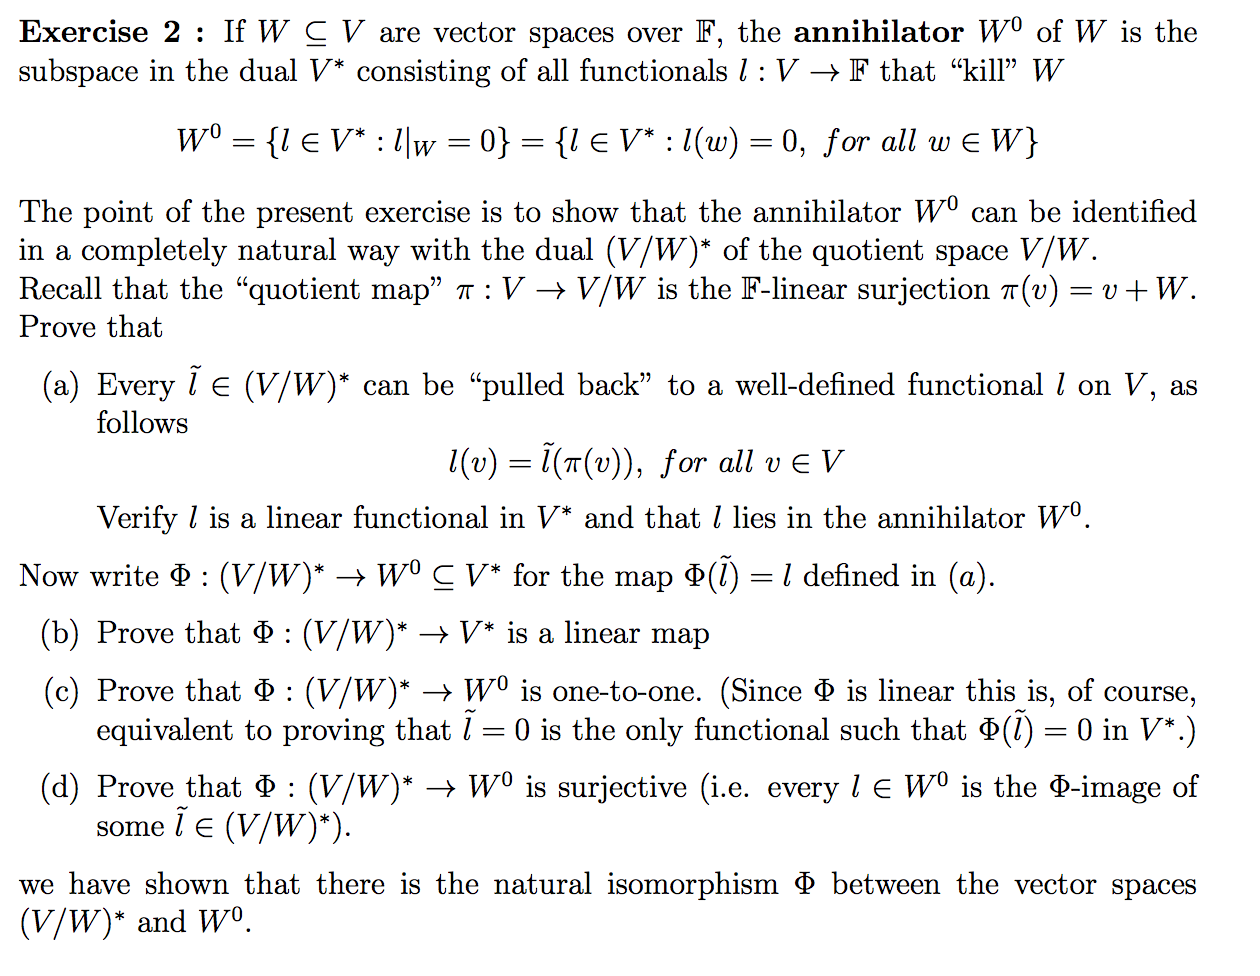
\includegraphics[width=1\textwidth]{LA-3-2.png}
\end{figure}
\end{question}
\begin{solution} \hfill \\
\textbf{(a)} We first show that $l$ is a linear functional. Let $v_1 , v_2 \in V$. 
By the linearity of $\tilde{l}$ and a fact about quotient space $v_1 + v_2 + W = 
(v_1 + W) + (v_2 + W)$, it follows that
\eQb
l(v_1 + v_2) &=& \tilde{l}(\pi(v_1 + v_2)) \\
&=& \tilde{l}( v_1 + v_2 + W ) \\
&=& \tilde{l}((v_1 + W) + (v_2 +W)) \\
&=& \tilde{l}(\pi(v_1) + \pi(v_2)) \\
&=& \tilde{l}(\pi(v_1)) + \tilde{l}(\pi(v_2)) \\
&=& l(v_1) + l(v_2). \\
\eQe
Let $\alpha \in \mathbb{F}$. Similarly, we have
\eQb
l(\alpha v) &=& \tilde{l}(\pi(\alpha v_1)) \\
&=& \tilde{l}(\alpha v_1 + W) \\
&=& \alpha \tilde{l}(v_1 + W) \\
&=& \alpha l(v). 
\eQe
Observe that for $w \in W$, as any linear functional sends origin to $0$, we have 
\eQb
l(w) &=& \tilde{l}(\pi(w)) \\
&=& \tilde{l}(W) \\
&=& 0.
\eQe
Therefore, we have shown that $l \in V^*$ and $l$ lies in the annihilator $W^0$.  

\bigskip

\textbf{(b)}For any $v \in V$, it follows that
\eQb
\Phi(\tilde{l}_1 + \tilde{l}_2)(v) &=& \tilde{l}_1 + \tilde{l}_2(\pi(v)) \\
&=& \tilde{l}_1(\pi(v)) + \tilde{l}_2(\pi(v)) \\
&=& \Phi(\tilde{l}_1)(v)  + \Phi(\tilde{l}_2)(v), \\ 
\eQe
which gives $\Phi(\tilde{l}_1 + \tilde{l}_2) = \Phi(\tilde{l}_1) + \Phi(\tilde{l}_2)$. 
Similarly, we have, for any $v \in V$, 
\eQb
\Phi(\alpha \tilde{l})(v) &=&  \alpha \tilde{l}(\pi v) \\
&=& \alpha \Phi(\tilde{l}).
\eQe
Therefore, $\Phi$ is linear. 

\bigskip

\textbf{(c)} Let $\tilde{l} \in (V\setminus W)^{*}$ such that $\Phi(\tilde{l}) = 0$. Then,
for $v \in V$, it follows that $\tilde{l}(\pi(v)) = 0$, thus $\tilde{l}(v + W) = 0$. Therefore,
$\tilde{l}$ is zero for any coset, hence $\tilde{l} = 0$. Therefore, $\Phi$ is injective.  

\bigskip

\textbf{(d)} Let $l \in W^0$. Now, let $\{v_{\lambda}\}$ be the coset representatives of
left cosets of $W$ in V. Define $\tilde{l} \in (V\setminus W)^*$ by
$\tilde{l}([v_\lambda]) = l(v_\lambda)$. Then, by definition of $\Phi$, we have that
$\Phi(\tilde{l}) = l$. Hence, we have shown that $\Phi$ is surjective. 

\hfill $\qed$

\end{solution}

\bigskip

\begin{question}[3]
\hfill
\begin{figure}[h!]
  \centering
    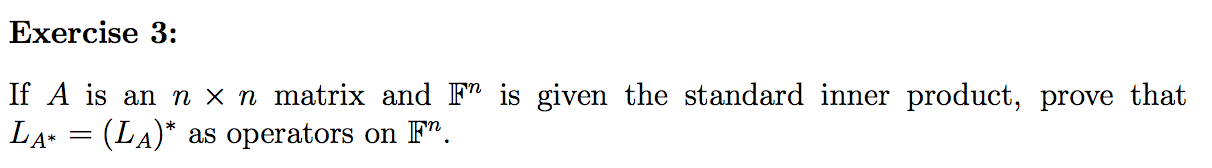
\includegraphics[width=1\textwidth]{LA-3-3.png}
\end{figure}
\end{question}
\begin{solution}
Let $B$ be the standard basis of $\mathbb{F}^n$. It follows that $[L_{A}]_{B} = A$,
and $L_{A^*}]_{B} = A^*$.  
Since $B$ is orthonormal basis of $\mathbb{F}^n$, we have that $[(L_{A})^*]_{B} = [L_{A}]_{B}^* = A^*$.
Hence, we obtain $[L_{A^*}]_{B} = [(L_{A})^*]_{B}$, thus $L_{A^*} = (L_{A})^*$ as required. 
\hfill $\qed$

\end{solution}

\bigskip

\begin{question}[4]
\hfill
\begin{figure}[h!]
  \centering
    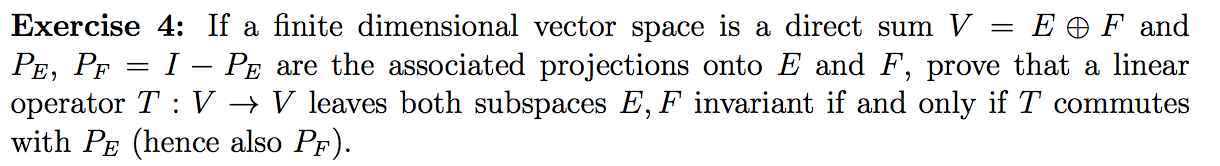
\includegraphics[width=1\textwidth]{LA-3-4.png}
\end{figure}
\end{question}
\begin{solution}
Assume that $T(E) \subset E$ and $T(F) \subset F$. Fix $x \in V$.
As $E$ and $F$ form a direct sum, we have $x = e + f$ for unique $e,f$ from $E$ and $F$ respectively.
By the invariance of the subspaces with respect to the $T$ operator, and the linearity of $T$
and $P_{E}$, it follows that
\eQb
T P_{E}(x) &=& T(e) \\ 
P_{E} T(x) &=& P_{E}(T(e) + T(f))  = P_{E}(T(e)) + P_{E}(T(f)) = T(e). \\
\eQe

Hence, it follows that $T P_{E} = P_{E} T$. 

\smallskip

Assume that $T P_{E} = P_{E} T$. It follows that
$T P_{E}(E) = P_{E} T (E)$. Since $P_{E}(E) = E$, we have $T(E) = P_{E}(T(E))$. As $P_{E}$ is a projection
onto $E$, this implies that $T(E) \subset E$. Hence, $T$ leaves $E$, and $F$ invariant. 
\hfill $\qed$ 
\end{solution}

\newpage

\begin{question}[5]
\hfill
\begin{figure}[h!]
  \centering
    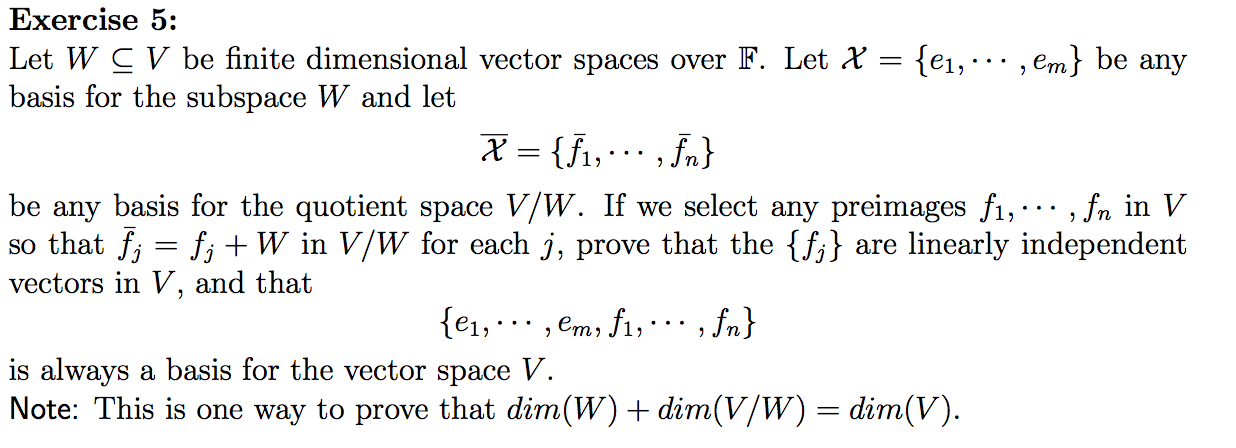
\includegraphics[width=1\textwidth]{LA-3-5.png}
\end{figure}
\end{question}
\begin{solution}
Let $\pi:V \to V\setminus W$ be the canonical projection map. 
We first show that $\{ f_1 , ..., f_n\} $ is linearly independent. Assume that
$\sum_{i=1}^{n} c_i f_i = 0$. By the linearity of $\pi$, it follows that
\eQb
\pi(\sum_{i=1}^{n} c_i f_i ) &=& \sum_{i=1}^{N} c_i \pi(f_i) \\
&=& \sum_{i=1}^{n} c_i \tilde{f_i}. 
\eQe
Since $\pi(0) = W$, we obtain
\eQb
W &=& \sum_{i=1}^{n} c_i \tilde{f_i}, 
\eQe
and by the linear independence of $\tilde{f_i}$s, we have that $c_1 = ...= c_n = 0$.
Hence, $\{ f_1, ..., f_n\}$ is linearly independent. Now, as $\{e_i\}$ and
$\{f_j\}$ are linearly independent from each other, it follows that $\{ e_1,...,f_n\}$.
We now show that the set spans $V$. Fix $v \in V$. Take $v + W$. Since $\{\tilde{f_j} \}$
are basis of the quotient space, we have that $v + W$ can be expressed as a linear combination
of $\{\tilde{f}_j\}$. Now, taking the pre-image it follows that $v - \sum c_j f_j \in W$. Therefore,
Using the $\{e_i \}$ we can express $v - \sum c_j f_j$ as a linear combination of them. Hence, 
this shows that an arbitrary element can be spanned by $\{ e_1, ... f_n \}$.
\hfill $\qed$ 

\end{solution}

\newpage

\begin{question}[6]
\hfill
\begin{figure}[h!]
  \centering
    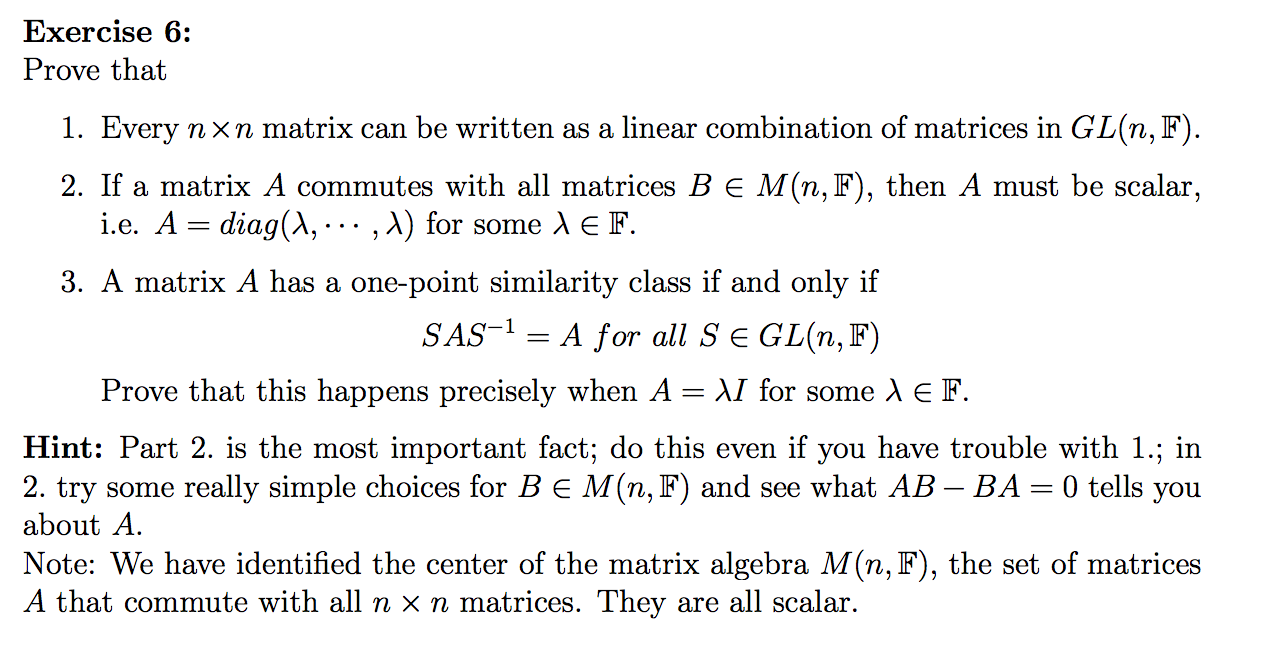
\includegraphics[width=1\textwidth]{LA-3-6.png}
\end{figure}
\end{question}
\begin{solution}
\textbf{(a)} We must show that $GL(n,\mathbb{F})$ spans $M(n,\mathbb{F})$.   

\bigskip

\textbf{(b)} Let $A \in M(n,\mathbb{F})$. Assume that $AB = BA$ for any $B \in M(n,\mathbb{F})$.
Let $E_{ij}$ be a matrix, where its $1$ at $(i,j)$ and $0$ elsewhere. Observe that
\eQnb 
A = \sum_{1 \leq k,l \leq n} a_{kl}E_{kl} \> &\text{ and }& \> E_{ij}E_{kl} = \delta_{jk} E_{il} ,
\label{eq:1} 
\eQne
for $1 \leq i,j,k,l \leq n$. As $A$ commutes with any matrix, and by $\eqref{eq:1}$, it follows that 
\eQb
0 &=& A E_{ij} - E_{ij}A \\
&=& (\sum_{1 \leq k,l \leq n} a_{kl}E_{kl}) E_{ij} - E_{ij}(\sum_{1 \leq k.l \leq n} a_{kl}E_{kl}) \\
&=& \sum_{k=1}^{n} a_{ki} E_{kj} - \sum_{l=1}^{n} a_{jl}E_{il} 
\eQe
\bigskip

\textbf{(c)} Let $A = \lambda I$. It follows that for any $S \in A$,
\eQb
SAS^{-1} &=& S\lambda I S^{-1} \\
&=& \lambda S I S^{-1} \\
&=& \lambda I = A. \\
\eQe
Now, let $A \in M(n,\mathbb{F})$ and assume that $SAS^{-1} = A$ for all $S \in GL(n,\mathbb{F})$.
Equivalently, we have $SA = AS$ for all $S \in GL(n,\mathbb{F})$. Now consider a matrix $B
\in M(n,\mathbb{F}$. By $(a)$, we have that $B = \sum_{i=1}^{n} c_i S_i$, for some $c_i$ and $S_i$
from $GL(n,\mathbb{F})$. It follows that 
\eQb
AB &=& A(\sum_{i=1}^{n} c_i S_i) = c_i \sum_{i=1}^{n} AS_i \\
&=& c_i \sum_{i=1}^{n} S_i A =  BA.
\eQe
Therefore, by $(b)$, we have that $A = \lambda I$ for some $\lambda \in \mathbb{F}$.
\hfill $\qed$


\end{solution}

\newpage

\begin{question}[7]
\hfill
\begin{figure}[h!]
  \centering
    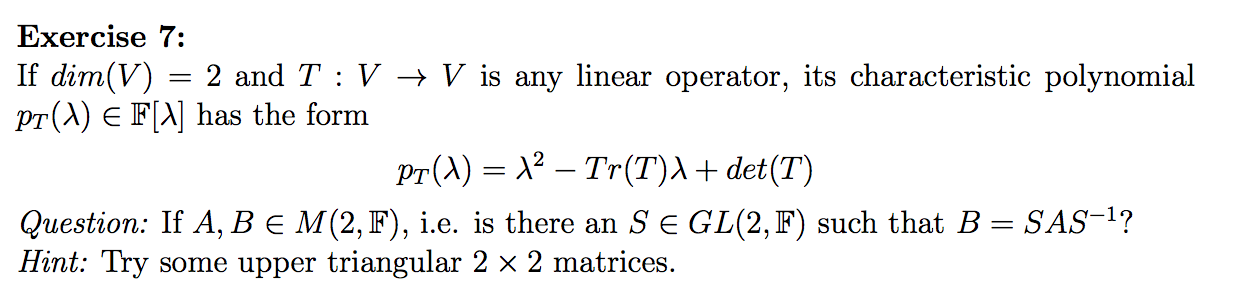
\includegraphics[width=1\textwidth]{LA-3-7.png}
\end{figure}
\end{question}
\begin{solution} 
It is a well-known result that one can determine the equivalence class of an $n \times n$ matrix
by looking at its real jordan form. In the case of $M(2,\mathbb{R})$, the forms are as follows:
\eQb
\begin{pmatrix} 
\lambda & 0 \\
0 & \mu \\
\end{pmatrix}, \> 
\begin{pmatrix}
\lambda & 1 \\
0 & \lambda \\
\end{pmatrix}, \text{ and }
\begin{pmatrix}
a & -b \\
b & a \\
\end{pmatrix},
\eQe
where the implication is that two matrices are similar if and only if they have the same real
jordan form. Hence, in the two by two case, we have identified 3 equvialence classes of matrix
similarity. \hfill $\qed$
\end{solution}


\end{document}
